%!TEX root = ./main.tex


\section{Intro}
\addtocounter{minutes}{2}
\begin{frame}
	\frametitle{Intro} 
	%\framesubtitle{}
    Initiatief van studenten
    
    \begin{figure}
       	\begin{minipage}{0.3\linewidth}
            \centering
           	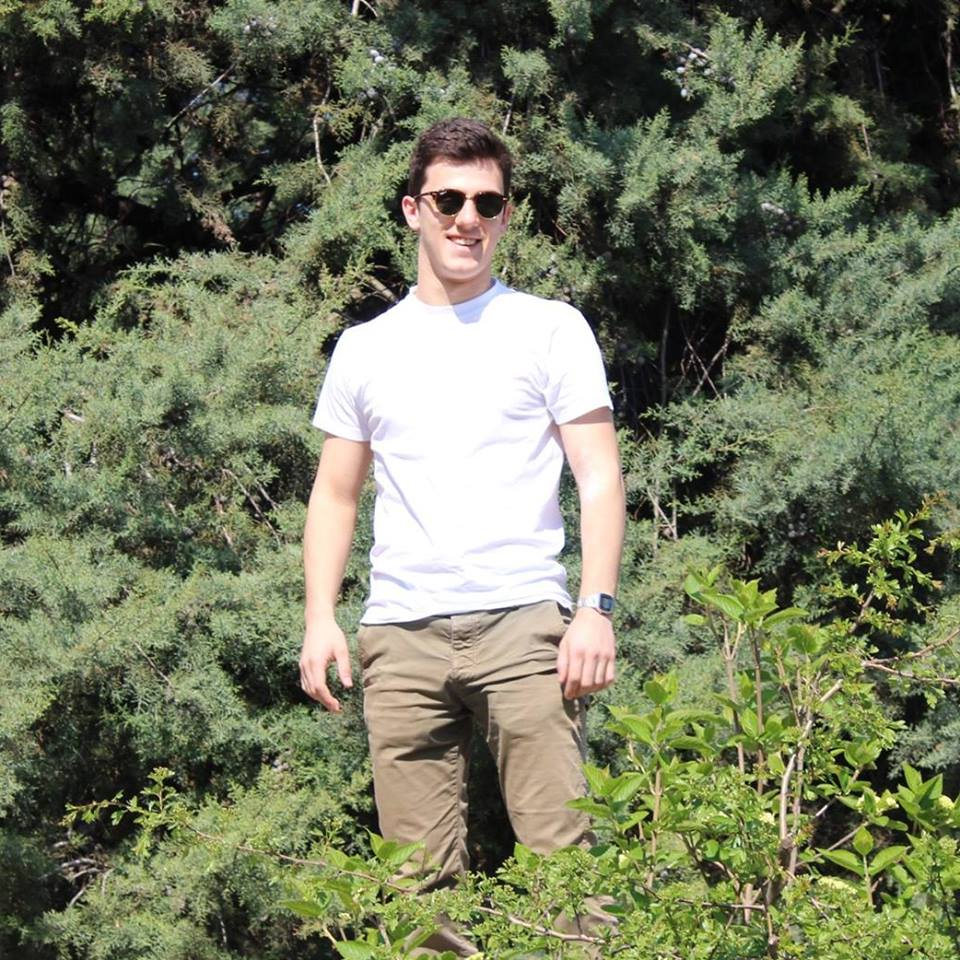
\includegraphics[width=\linewidth]{res/andrei} \\
           	\footnotesize Andrei Bondarenko
        \end{minipage}
        \begin{minipage}{0.3\linewidth}
           	\centering
			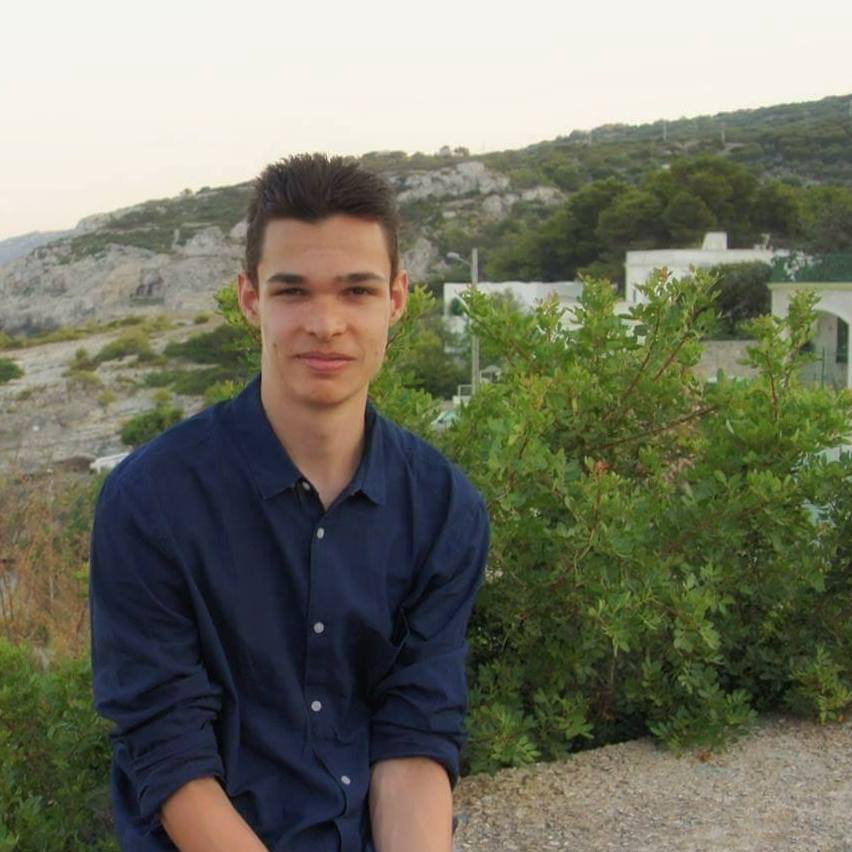
\includegraphics[width=\linewidth]{res/stijn} \\
           	\footnotesize Stijn Rosaer
       	\end{minipage}
        \begin{minipage}{0.3\linewidth}
           	\centering
			
\includegraphics[width=\linewidth]{res/igor} \\
           	\footnotesize Igor Schittekat 
       	\end{minipage}
        \begin{minipage}{0.3\linewidth}
           	\centering
			
\includegraphics[width=\linewidth]{res/joey} \\
           	\footnotesize Joey De Pauw
       	\end{minipage}
        \begin{minipage}{0.3\linewidth}
           	\centering
			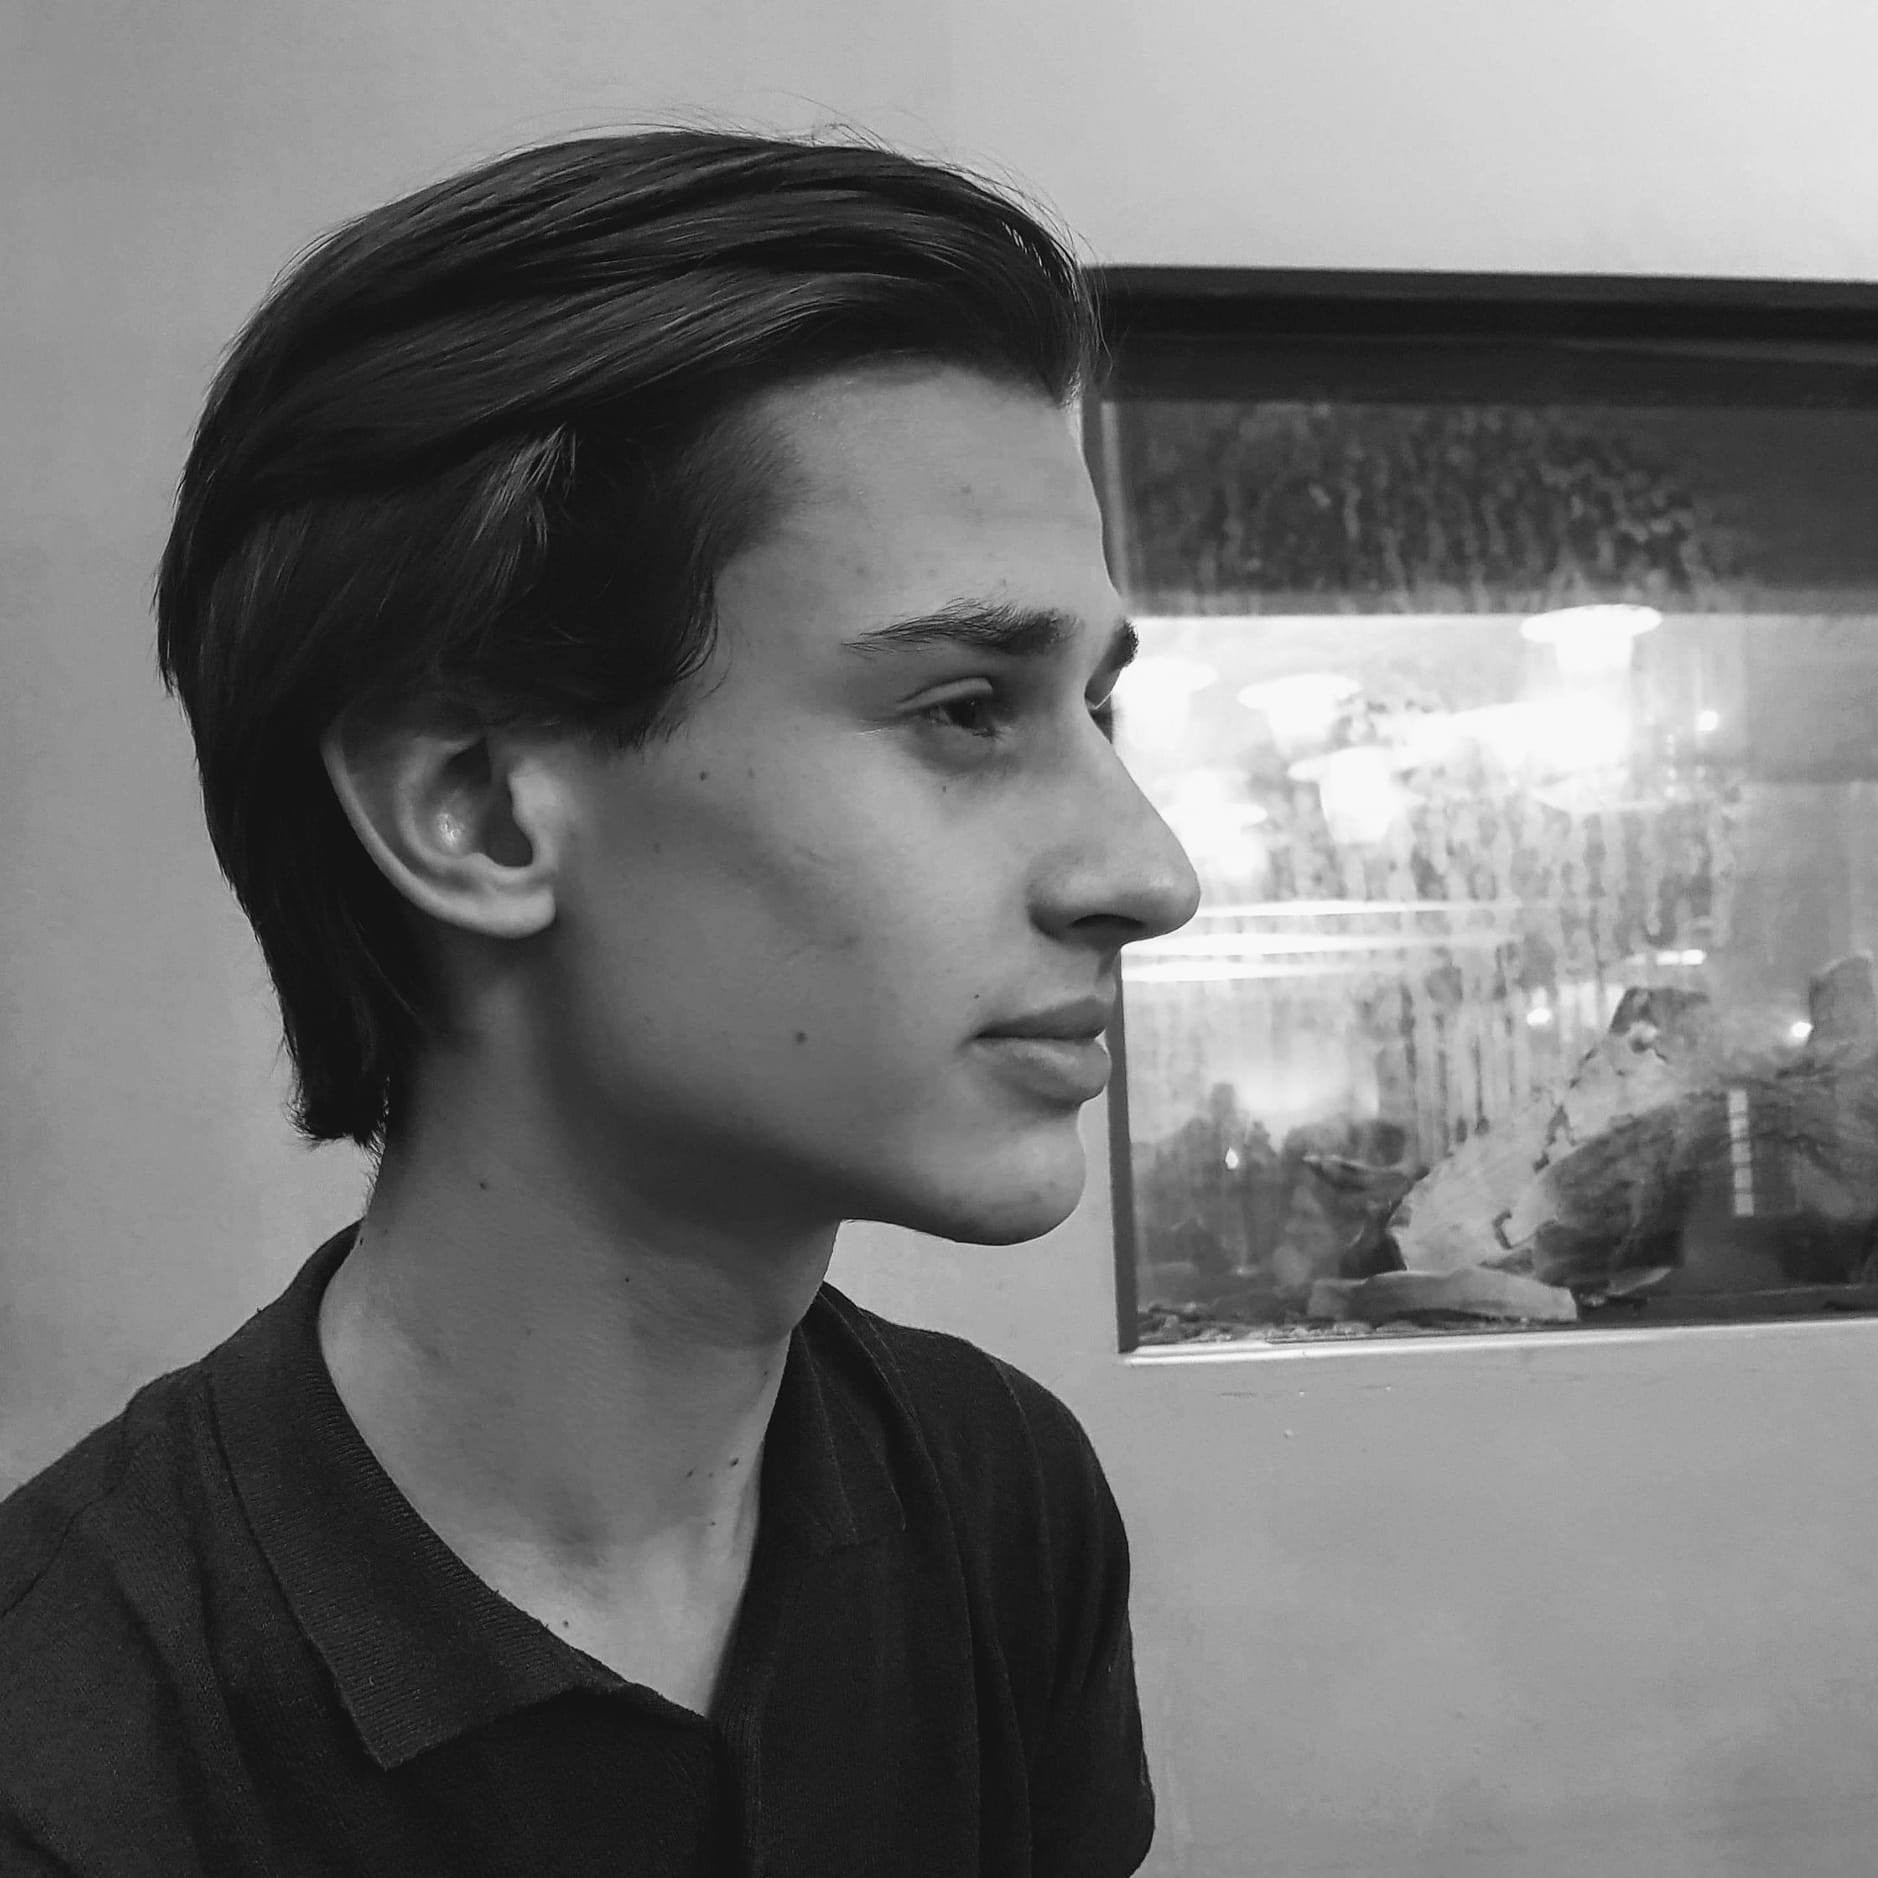
\includegraphics[width=\linewidth]{res/senne} \\
           	\footnotesize Senne Rosaer
       	\end{minipage}
        \begin{minipage}{0.3\linewidth}
           	\centering
			
\includegraphics[width=\linewidth]{res/toon} \\
           	\footnotesize Toon Meynen
       	\end{minipage}
    \end{figure}

\end{frame}  
   
    
\section{Planning}
\addtocounter{minutes}{3}
\begin{frame}
	\frametitle{Planning}
    \includeSchedule
    
	% NOTE: Volgende sessie:  Dual boot $->$ USB stick en laptop

\end{frame}

\section{WINAK}
\begin{frame}
	\frametitle{WINAK}
	\framesubtitle{\textbf{W}iskunde \textbf{I}nformatica \textbf{Na}tuurkunde \textbf{K}ring}
    
    \begin{itemize}
        \item\link{https://www.facebook.com/groups/2156957474519310/}{Facebook Groep}
        \item\link{https://forum.winak.be/}{Forum}
        \item\link{http://tuyaux.winak.be/}{Tuyaux}
        \item Lidkaart
        \item Mentoren
        \begin{itemize}
           	\item\link{https://www.facebook.com/elise.verlinden.9} {Elise (Wiskunde)}
           	\item\link{https://www.facebook.com/profile.php?id=100009929418782} {Thomas (Fysica)}
			\item\link{https://www.facebook.com/toon.meynen.3} {Toon (Informatica)}
		\end{itemize}
		\item Doop
        \item\link{https://www.facebook.com/events/243230606368223/}{Openings Cafe Avond}
        
	\end{itemize}

\end{frame}
    
%     \section{Blackboard \& SiSa}
% 	\begin{frame}
% 		\frametitle{Blackboard}
% 		\framesubtitle{https://blackboard.uantwerpen.be}
%         \begin{itemize}
%         \item Facebook van de universiteit
%           \begin{itemize}
%             \item Updates
%             \item Projecten
%             \item Oefeningen
%           \end{itemize}
% 		\end{itemize}
% 	\end{frame}
	
% 	\begin{frame}
% 		\frametitle{SiSa}
% 		\framesubtitle{https://sisastudent.uantwerpen.be}
%         \begin{itemize}
%           \item Administratie van de universiteit
%           \begin{itemize}
%             \item Inschrijven
%             \item Lessenrooster
%             \item Rekeningen
%           \end{itemize}
% 		\end{itemize}
% 	\end{frame}
    
\section{Email \& Lessenrooster}
\begin{frame}
	\frametitle{Email}
	\framesubtitle{https://mail.student.uantwerpen.be}
    \begin{center}
       	\tcbox[colback=white, colframe=darkblue]{
           	\parbox{7.5cm}{
              \centering
              s018xxxx@ad.ua.ac.be OF \\
              voornaam.achternaam@student.uantwerpen.be
            }
        }
    \end{center}
   	\textbf{IMAP (inkomend)}
    \begin{tabularx}{\linewidth}{rX}
      Server name & outlook.office365.com \\
      Port & 993 \\
      Encryption & SSL \\
	\end{tabularx} \vspace{0.5cm}
    
	\textbf{SMTP (uitgaand)}
    \begin{tabularx}{\linewidth}{rX}
      Server name & smtp.office365.com \\
      Port & 587 \\
      Encryption & STARTTLS \\
	\end{tabularx} \vspace{0.5cm}
    
   % NOTE: mogelijk dient u poort 143 te gebruiken bij de IMAP instellingen, wanneer het niet meteen lukt om met bovenstaande gegevens uw e-mail binnen te halen.
\end{frame}
    
\begin{frame}
	\frametitle{Lessenrooster}
	%\framesubtitle{}
	
	\link{https://www.sisa.uantwerpen.be}{SiSa}
	\vspace{0.5cm}
	
    \begin{itemize}
    	  \item SiSa $\rightarrow$ rooster $\rightarrow$ abonneer op rooster
      \item Agenda toevoegen via url
    \end{itemize}
    
    %TODO: Include screenshots
    
\end{frame}

\section{Cursusdienst \& Printen}
\begin{frame}[allowframebreaks=10]
	\frametitle{Cursusdienst}
	%\framesubtitle{}
    \link{https://www.uantwerpen.be/nl/onderwijs/studerenuantwerpen/starten-als-student/colleges-cursussen-examens/cursusdienst/}{Website UA - Cursusdienst}
    \vspace{0.5cm}
    
    Tips:
    \begin{itemize}
        \item Verplicht $\neq$ Verplicht Verplicht
        \item Cursussen zeker kopen
        \item Handboeken ter referentie
        \item Schrijf de nummers van de cursussen en handboeken op
	\end{itemize}
    
	% NOTE:
	% Verplicht = sterk aangeraden door prof
	% Cursussen: relatief goedkoop, soms op examens gebruiken
	% Handboeken: duurder, meer achtergrond info, kan handig zijn

    
    \framebreak
    \begin{figure}
       	\centering
        \vspace*{0.02cm}
        \textbf{Campus Groenenborger} \\
        \vspace{0.3cm}
       	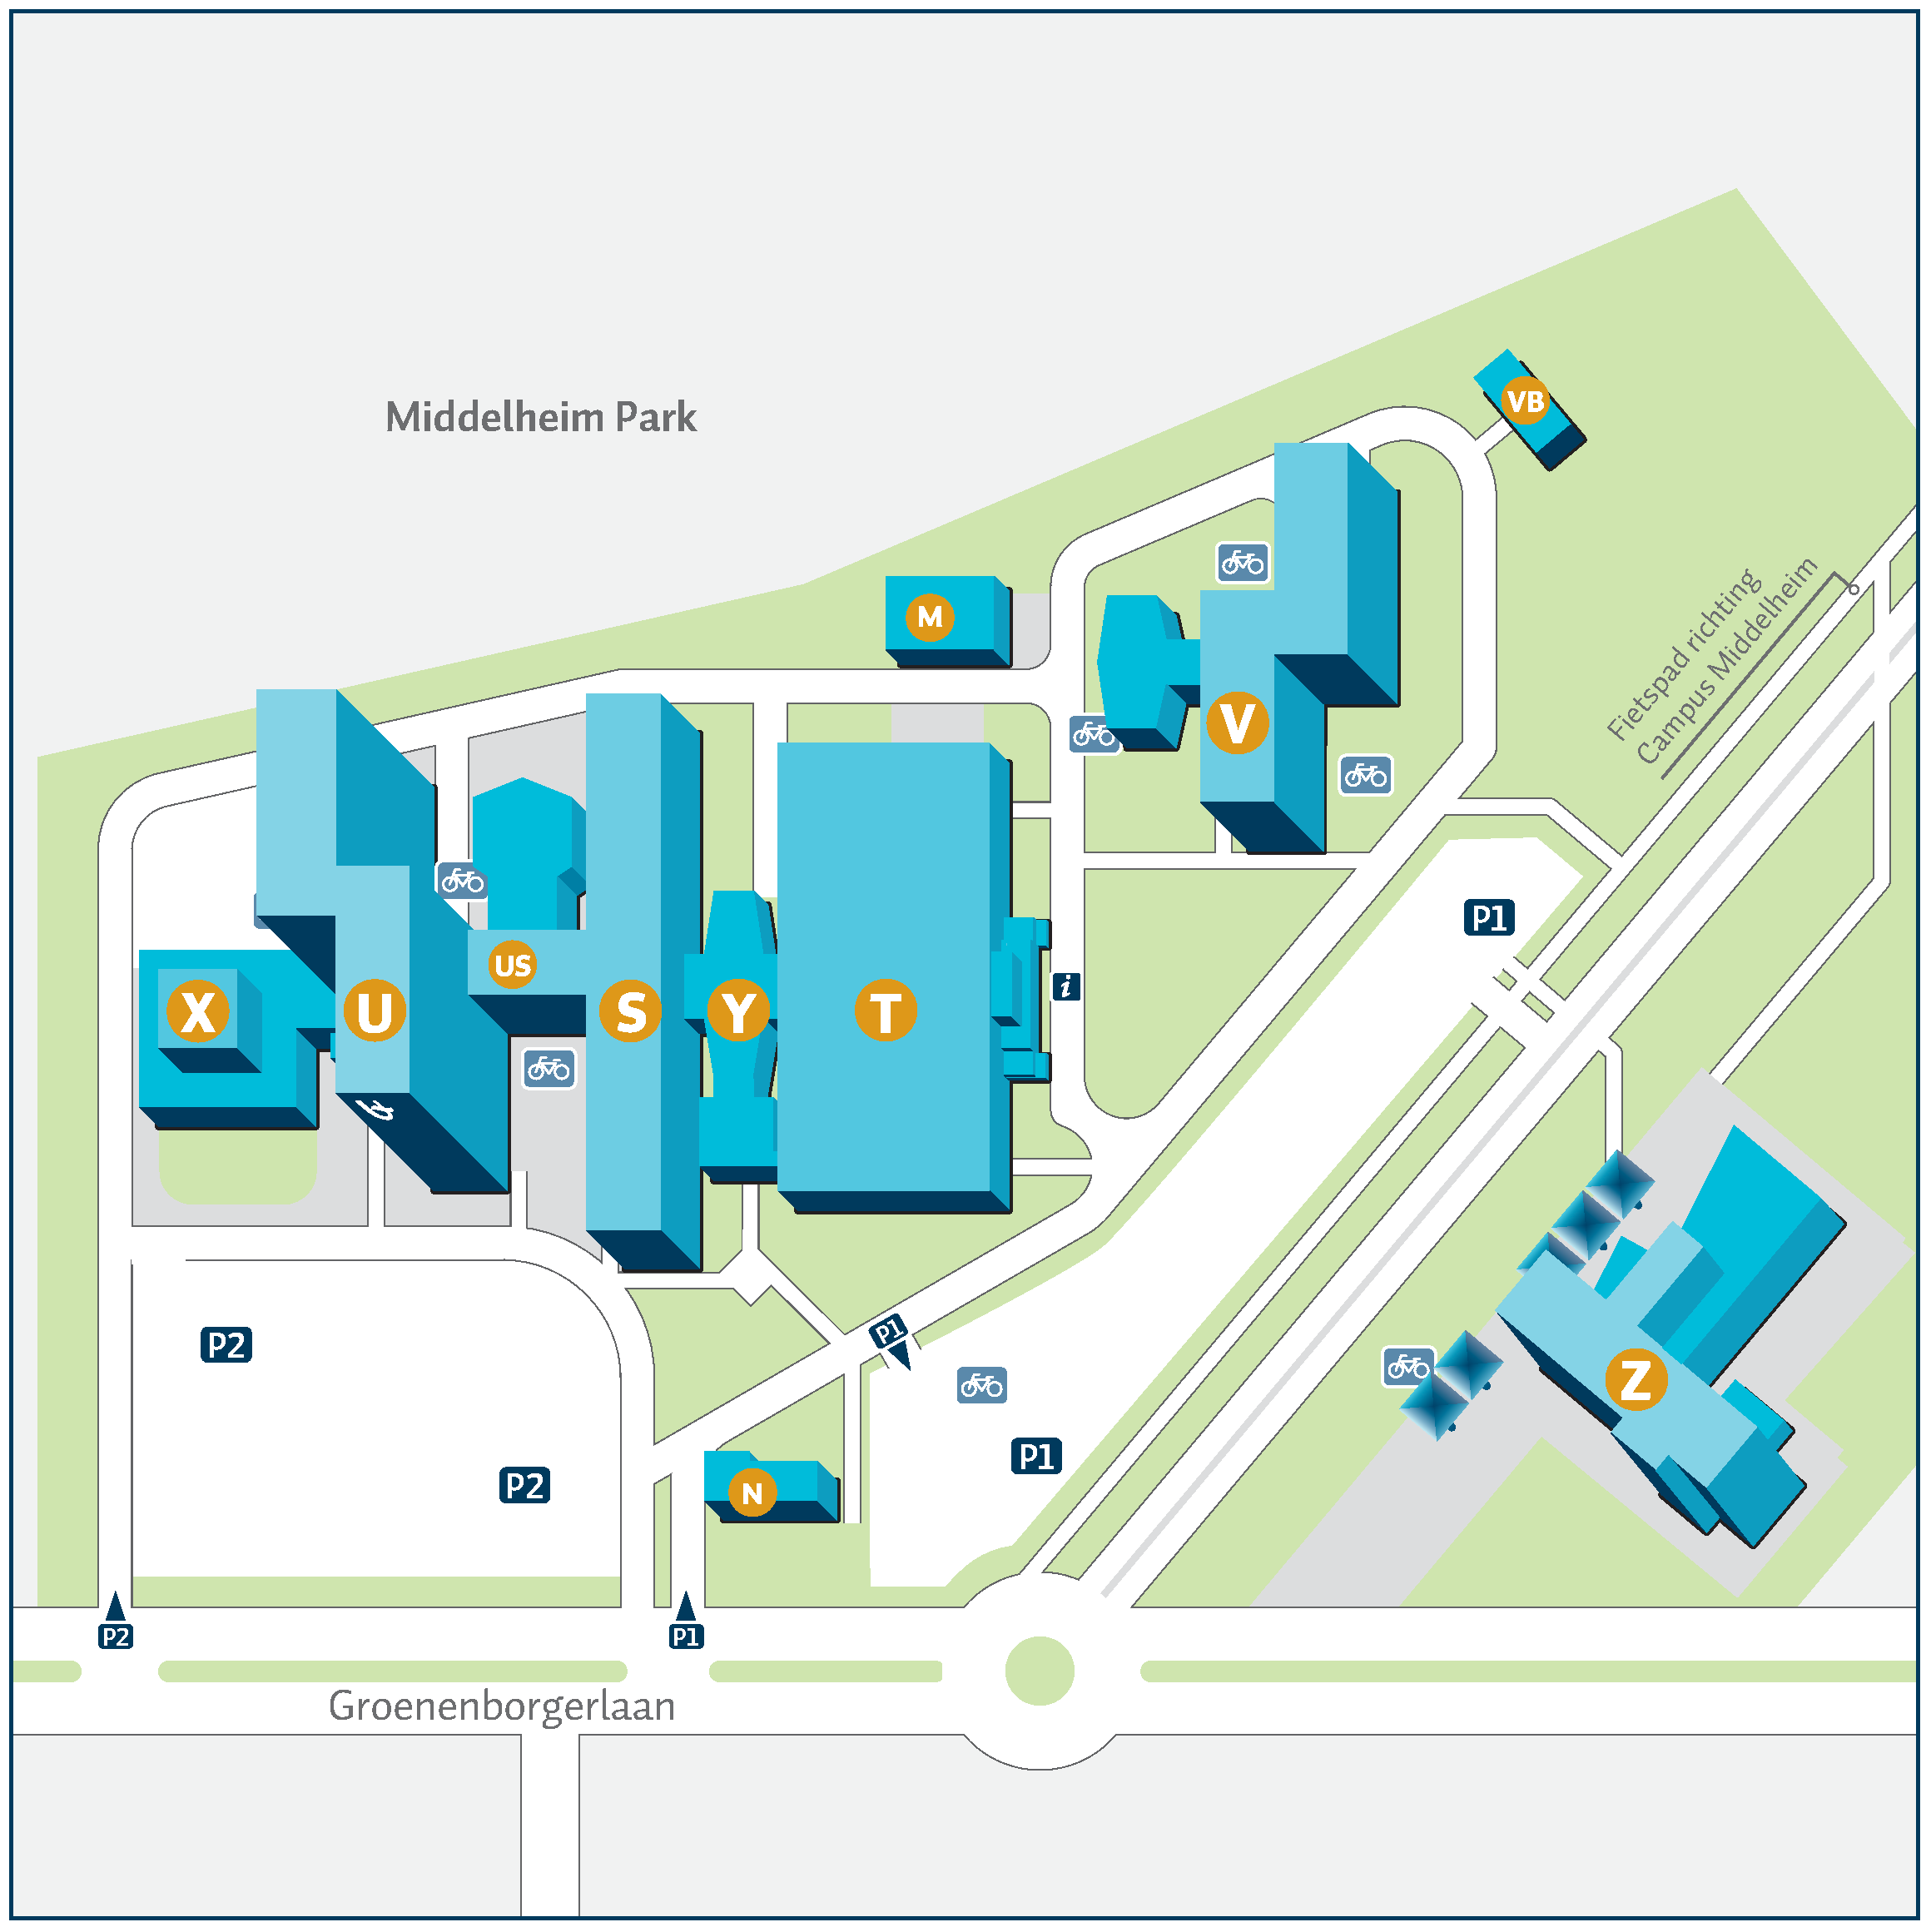
\includegraphics[width=0.65\linewidth]{res/CGB}
    \end{figure}
    \framebreak
    \begin{figure}
       	\centering
        \vspace*{0.02cm}
        \textbf{Cursusdienst Campus Groenenborger U027} \\
        \vspace{0.3cm}
      		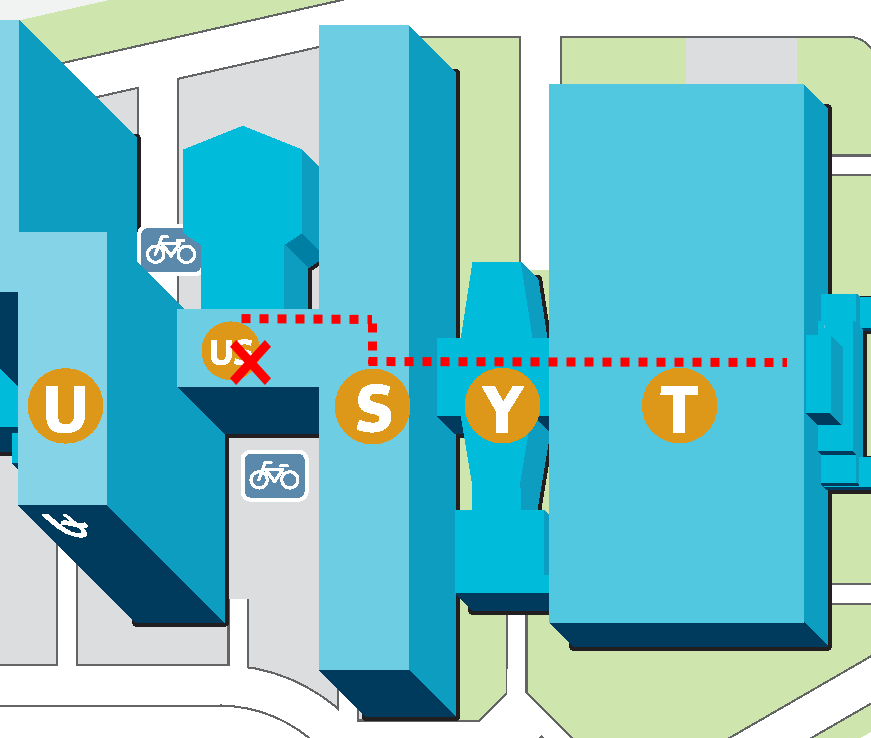
\includegraphics[width=0.8\linewidth]{res/CGB_CD_small}
    \end{figure}
\end{frame}

\begin{frame}[allowframebreaks=10]
	\frametitle{Printen}
	% framesubtitle{}
    
    \link{https://www.uantwerpen.be/nl/bibliotheek/diensten/faciliteiten/ter-plaatse/printen-kopieren-scannen/}{Website UA - Printen}
    \vspace{0.5cm}
    
    \begin{enumerate}
       	\item Maak een printaccount aan
        \item Koop een betaalkaart aan een verdeelautomaat (€ 2)
        \item Laad de betaalkaart online op (min € 5 - max € 50)
        \item  Ga naar een kopieertoestel en koppel je printaccount aan de betaalkaart
        \item Printen
    \end{enumerate}
%         \framebreak
%         \begin{figure}
%         	\centering
%             \vspace*{0.02cm}
%             \textbf{Bibliotheek Campus Groenenborger} \\
%             \vspace{0.3cm}
%        		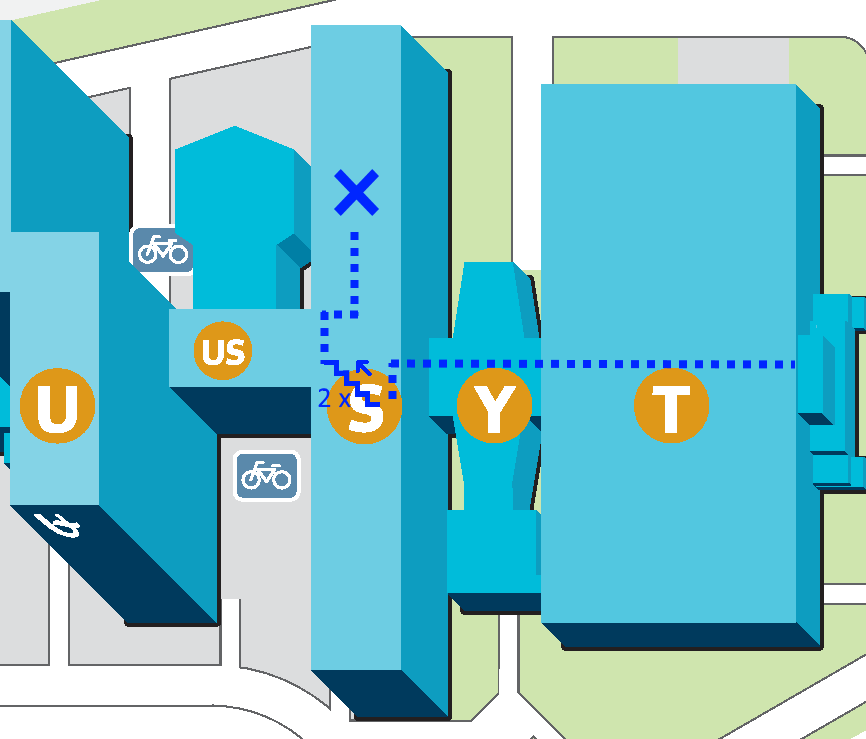
\includegraphics[width=0.8\linewidth]{res/CGB_BIB_small}
%         \end{figure}
\end{frame}

\section{Rondleiding \& Receptie}
\begin{frame}
	\frametitle{Rondleiding \& Receptie}
	\framesubtitle{Sponsored by WINAK}
    \begin{itemize}
       	\item Gebouw G
        \item Leercentrum ``De Parabool''
        \item PC Labo
        \item Free Drinks
	\end{itemize}
\end{frame}
